\appendix
\section{Projection Details}\label{Sec:Projection}
To enforce the divergence constraint in {\bf Step 3, 7}, and {\bf 11}, we use a projection method analgous to the methods originally developed for incompressible flow \citep{almgren1998conservative,bell1989second}.
The basic idea is to decompose the velocity field into a divergence-free component and a curl-free (gradient of a scalar field) component by solving a variable-coefficient Poisson equation for the scalar field.
The details for the MAC projection in {\bf Step 3} and {\bf Step 7} are given in Appendix B of Paper III.  The details of the nodal projection in {\bf Step 11} are given in Section 3.2 of Paper III.
We note that in the nodal projection, the gradient of the scalar field is used to update the perturbational pressure, $\pi$.

Based on our past experience in the MAESTRO project, we have found it useful to split the velocity dynamics into a perturbational and base state velocity,
\begin{equation}
\Ub = \Ubt(\xb,t) + w_0(r,t)\eb_r,
\end{equation}
solve for each term separately, and immediately combine them to find a full velocity that satisfies the constraint.  We take that approach here, primarily because it allows us to enforce a boundary condition on $w_0$ at the edge of the star (i.e., the cutoff density location where we hold density constant).  Namely, to enforce that $r^2 w_0$ remain constant is difficult to do when solving for the full velocity. 
This is demonstrated in Figure \ref{fig:wdconvect_splitU} (right) where the velocity magnitude is observed to incorrectly increase outside the cutoff density radius when we use the full velocity in the nodal projection. The resulting peak temperature also dips significantly as seen in Figure \ref{fig:wdconvect_splitU} (left).   

%%%%%%%%%%%%%%%%%%%%%%%%%%%%%
\begin{figure}[htb]
\begin{center}
\begin{tabular}{l c}
\multirow{4}{3.25in}[30mm]{ 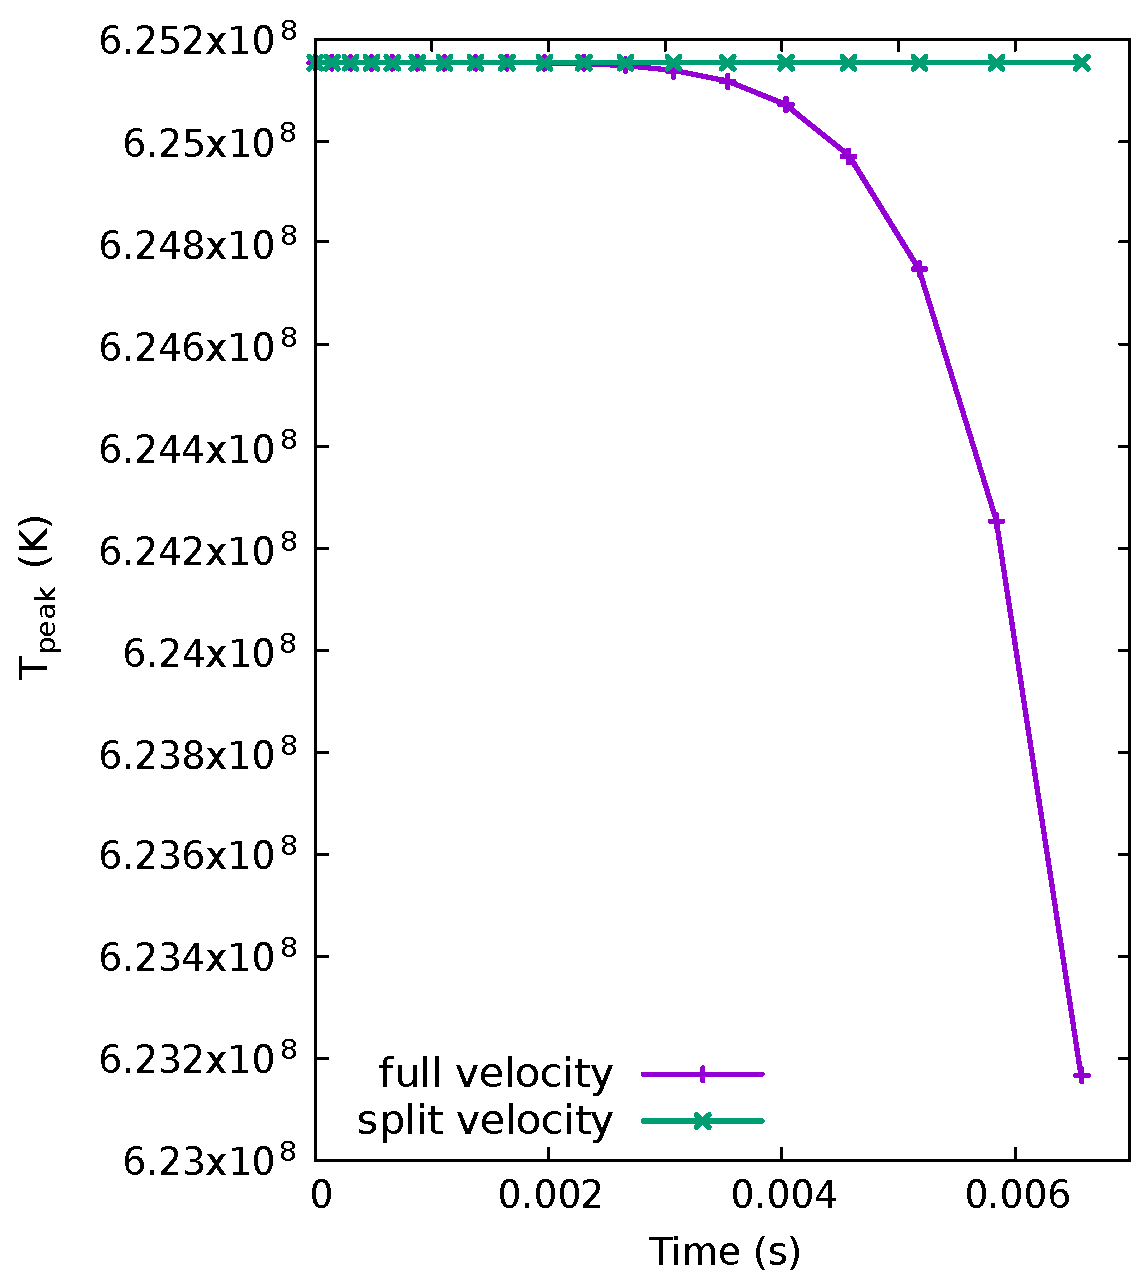
\includegraphics[width=3.0in]{./figs/wdconvect_256_splitU} } & \multicolumn{1}{c}{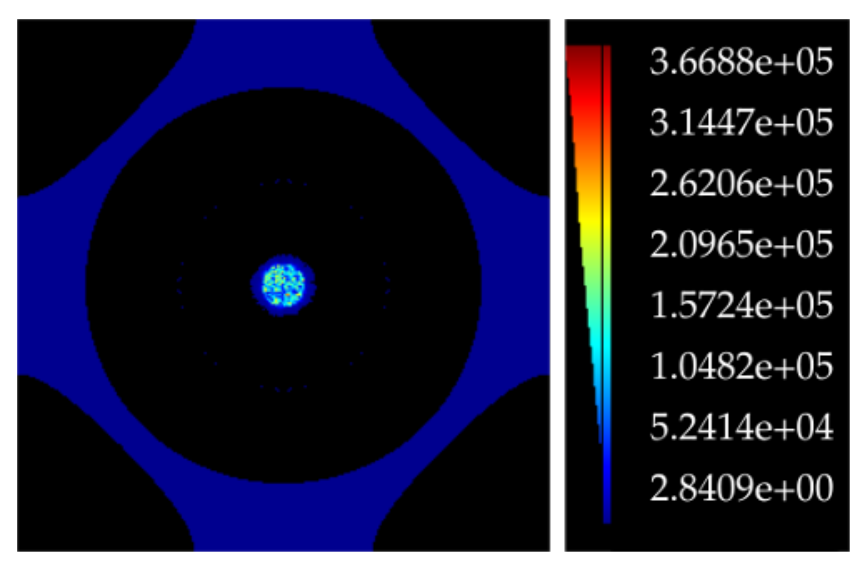
\includegraphics[width=2.35in]{./figs/magvel_full_XY}} \\
& \multicolumn{1}{c}{\begin{footnotesize} (a) Velocity magnitude, solved using full $\mathbf{U}$ \end{footnotesize}} \\[1.em]
& \multicolumn{1}{c}{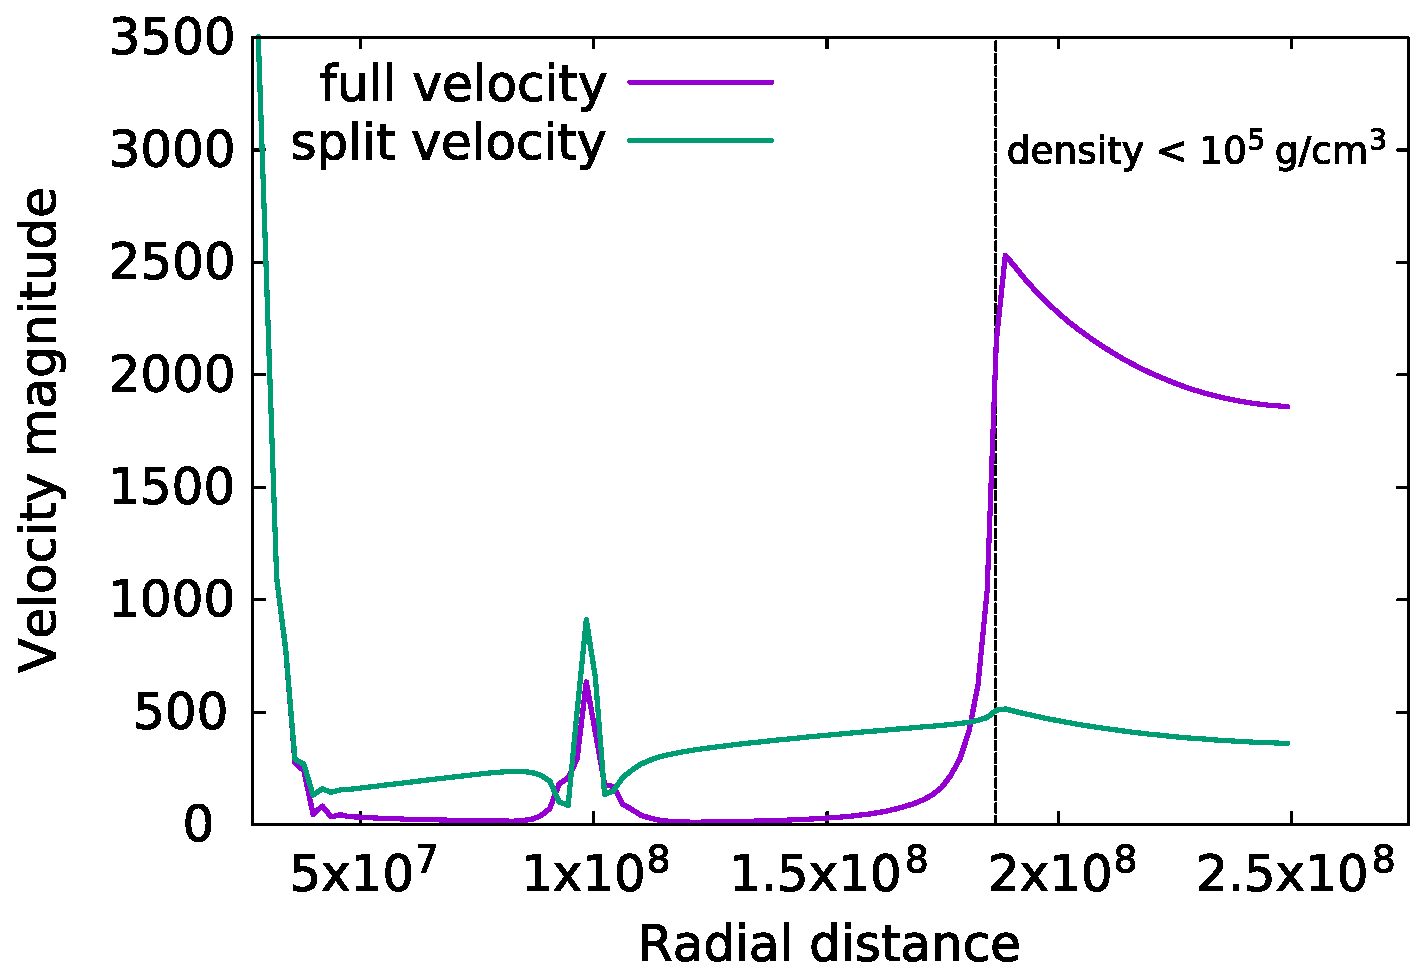
\includegraphics[width=2.75in]{./figs/magvel_lineout_X}} \\ 
& \multicolumn{1}{c}{\begin{footnotesize} (b) Comparison along white line \end{footnotesize}} \\
\end{tabular}
\caption{\label{fig:wdconvect_splitU} (Left) Peak temperature, $T_{\text{peak}}$ in a white dwarf at resolution of $256^3$ 
         during initial transition. (Right) Velocity magnitude solved using full velocity $\mathbf{U}$ in the projection step 
         results in much larger values outside the density cutoff region, $\rho < 10^5 \text{ g cm}^{-3}$, that is not seen when 
         we split the velocity dynamics.}
\end{center}
\end{figure}
%%%%%%%%%%%%%%%%%%%%%%%%%%%%%

So in practice, we solve the constraint over the lateral average,
\begin{equation}
\nabla\cdot\left(\beta_0\Ubt\right) = \beta_0(S-\overline{S})
\end{equation}
and separately solve for $w_0$ using 
\begin{equation}
\nabla\cdot(\beta_0w_0\eb_r) = \beta_0\left(\overline{S} - \frac{1}{\gammaonebar p_0}\frac{\partial p_0}{\partial t}\right).
\end{equation}
To solve for $\Ubt$ we use a projection method, which involves the solution of a variable-coefficient Poisson solver to extract the curl-free component of the unprojected velocity.
Note that MAESTRO contains alternate low Mach number formulations that conserve total energy in stratified systems, with minimal changes to the code (see Appendix A of \cite{subChandra_II} for details).
To find $w_0$ we integrate in 1D using the procedure in Appendix B of Paper V, keeping in mind that the base state spacing ($\Delta r$) should be computed using the appropriate cell-edge and cell-center locations when using irregularly-spaced base state.
Note that in this approach, we estimated the time-derivative of the pressure in part by examining how laterally averaged $\rho'=\rho-\rho_0$ changed over time (quantified by $\eta_\rho = \overline{\rho'\Ub\cdot\eb_r}$).  After evolving the species ({\bf Steps 4A/8A}), we compute this term in a similar fashion as reported in Paper V with the slight difference in using the full velocity instead of the split velocities. For example, after {\bf Step 8A}, we define a radial cell-centered $\etarho^{\nph}$, 

\begin{description}
\item For planar geometry, $\etarho = \overline{\rho'(\Ub\cdot\eb_r)}$,
\begin{equation}
 \etarho^{\nph} =  {\rm {\bf Average}} \sum_k \left[ \left(\uadvtwo \cdot \eb_r \right) (\rho X_k)^{\nph,\pred} \right]
\end{equation}
\item For spherical geometry, first construct 
$\etarho^{{\rm cart},\nph} = [\rho'(\Ub\cdot\eb_r)]^{\nph}$ on Cartesian cell centers using:
\begin{equation}
\etarho^{{\rm cart},\nph} = \left[\left(\frac{\rho^{(1)}+\rho^{(2)}}{2}\right)-\left(\frac{\rho_0^n+\rho_0^{n+1}}{2}\right)\right] \cdot \left( \uadvtwo \cdot \eb_r \right).
\end{equation}
Then,
\begin{equation}
\etarho^{\nph,\star} = {\rm {\bf Average}}\left(\etarho^{{\rm cart},\nph}\right).
\end{equation}
\end{description}



